\documentclass[journal=jacsat,manuscript=article]{achemso}
\usepackage[utf8]{inputenc}
\usepackage[T1]{fontenc}       % Use modern font encodings
\usepackage{amssymb}
\usepackage[version=3]{mhchem} % Formula subscripts using \ce{}
\usepackage{siunitx}
\usepackage[table]{xcolor}

\usepackage{xr,xc}
\externaldocument[M-]{ion_pairing_paper}
\externalcitedocument{ion_pairing_paper}

% Hack for making figures Say \figurename S\thefigure, e.g. Figure S1:
\makeatletter
\makeatletter \renewcommand{\fnum@figure}
{\textbf{Figure~S\thefigure}}
\makeatother

\renewcommand{\thetable}{\arabic{table}}
\makeatletter
\makeatletter \renewcommand{\fnum@table}
{\textbf{Tab.~S\thetable}}
\makeatother



\author{Hassan Srour}
\affiliation[Laboratoire de Chimie de l'ENS de Lyon]{Laboratoire de Chimie UMR CNRS 5182 Ecole Normale Supérieure de Lyon/ Université Claude Bernard Lyon1/ Université de Lyon 46 Allée d'Italie, 69007 Lyon}


\author{Mathieu Leocmach}
\affiliation[Institut Lumière Matière]{Institut Lumière Matière, CNRS UMR 5306, Université Claude Bernard Lyon 1, Université de Lyon, Lyon, 69622 Villeurbanne Cedex, France}
\email{mathieu.leocmach@univ-lyon1.fr}

\author{Martien Duvall Deffo Ayagou}
\author{Thi Thanh-Tam Nguyen}
\affiliation[Laboratoire de Chimie de l'ENS de Lyon]{Laboratoire de Chimie UMR CNRS 5182 Ecole Normale Supérieure de Lyon/ Université Claude Bernard Lyon1/ Université de Lyon 46 Allée d'Italie, 69007 Lyon}

\author{Nicolas Taberlet}
\author{Sébastien Manneville}
\affiliation[Laboratoire de Physique de l'ENS de Lyon]{Laboratoire de Physique, Ecole Normale Supérieure de Lyon/ Université Claude Bernard Lyon1/ Université de Lyon, 46 Allée d'Italie, 69007 Lyon}


\author{Chantal Andraud}
\author{Cyrille Monnereau}
\affiliation[Laboratoire de Chimie de l'ENS de Lyon]{Laboratoire de Chimie UMR CNRS 5182 Ecole Normale Supérieure de Lyon/ Université Claude Bernard Lyon1/ Université de Lyon 46 Allée d'Italie, 69007 Lyon}
\email{cyrille.monnereau@ens-lyon.fr}

%\title{Supramolecular crocodile line controls the rheological properties of polyelectrolytes hydrogels}
\title{Supplementary Informations to Ion pairing controls rheological properties of ``crocodile-line'' polyelectrolyte hydrogels}
%\title{Ion pairing in crocodile line hydrogels controls rheological properties}
%\title{In crocodile line hydrogels ion pairing controls rheological properties}
%\title{Controlling the rheological properties of well-defined polyelectrolytes hydrogels by fine tuning their ion pairing process}


\keywords{ATRP, hydrogel, poly(cations), rheology}

\begin{document}

%\section{Materials and methods}
All reactions were performed under an argon atmosphere using schlenk techniques. CH2Cl2 and THF were dried and degassed on a solvent station by passage through an activated alumina column followed by argon flush. All other solvents were used without additional purification. HEA purchased from Alfa Aesar was purified as reported in Ref~\cite{Srour2014} of the main text. Additional chemicals were obtained from Sigma Aldrich, Acros or Alfa Aesar and underwent no further purification. 

SEC analyses were carried out on ca \SI{5}{\milli\gram\per\milli\litre} solutions of each polymer in DMSO LiBr (\SI{0.01}{M}), using a MALVERN VISCOTEK 430  system equipped with three PSS Gram columns (Polyester Copolymer Network) set in series at \SI{80}{\celsius}, coupled to a Viscotek HT-GPC Module 350 A (refractive and viscosimeter) detector (at \SI{80}{\celsius}) . The polydispersity indexes (PDI = Mw/Mn) of the samples were derived from the RI signal by a universal calibration curve by pullulan. The number-average molar masses (Mn) were calculated from RI signals with the OmniSEC 4.6 software.

The high resolution mass spectra (MS QTOF) were recorded in positive and negative ion modes on a hybrid quadrupole time-of-flight mass spectrometer (MicroTOFQ-II, Bruker Daltonics, Bremen) with an electrospray ionization (ESI) ion source. The gas flow of the spray gas is \SI{0.6}{\bar} and the capillary voltage is $\pm\SI{4.5}{\kilo\volt}$. The solutions are infused at \SI{180}{\micro\litre\per\hour}. The mass range of the analysis is 50-1000~m/z and the calibration was done with sodium formate.

\begin{figure}
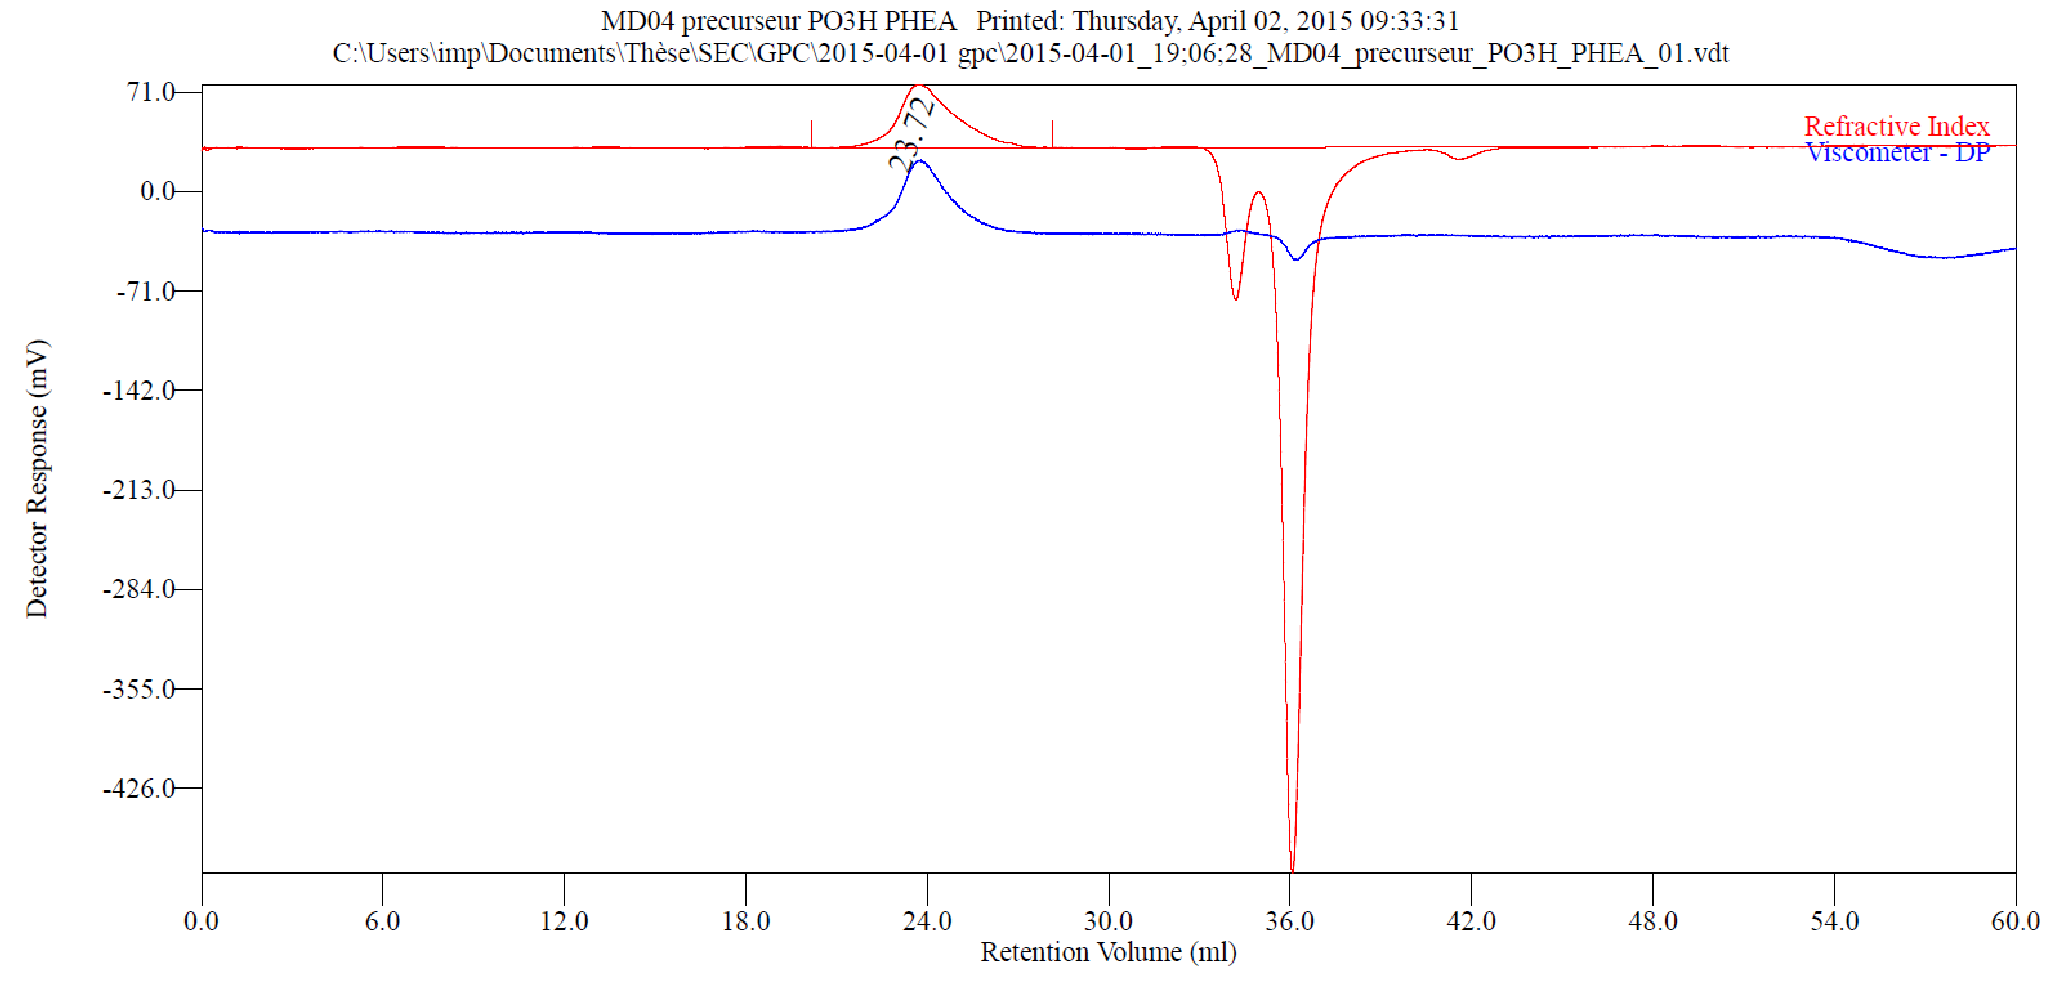
\includegraphics[width=\textwidth]{sec_spectra.png}
\caption{SEC Spectra of \ce{POH}.}
\label{fig:sec}
\end{figure}

\begin{figure}
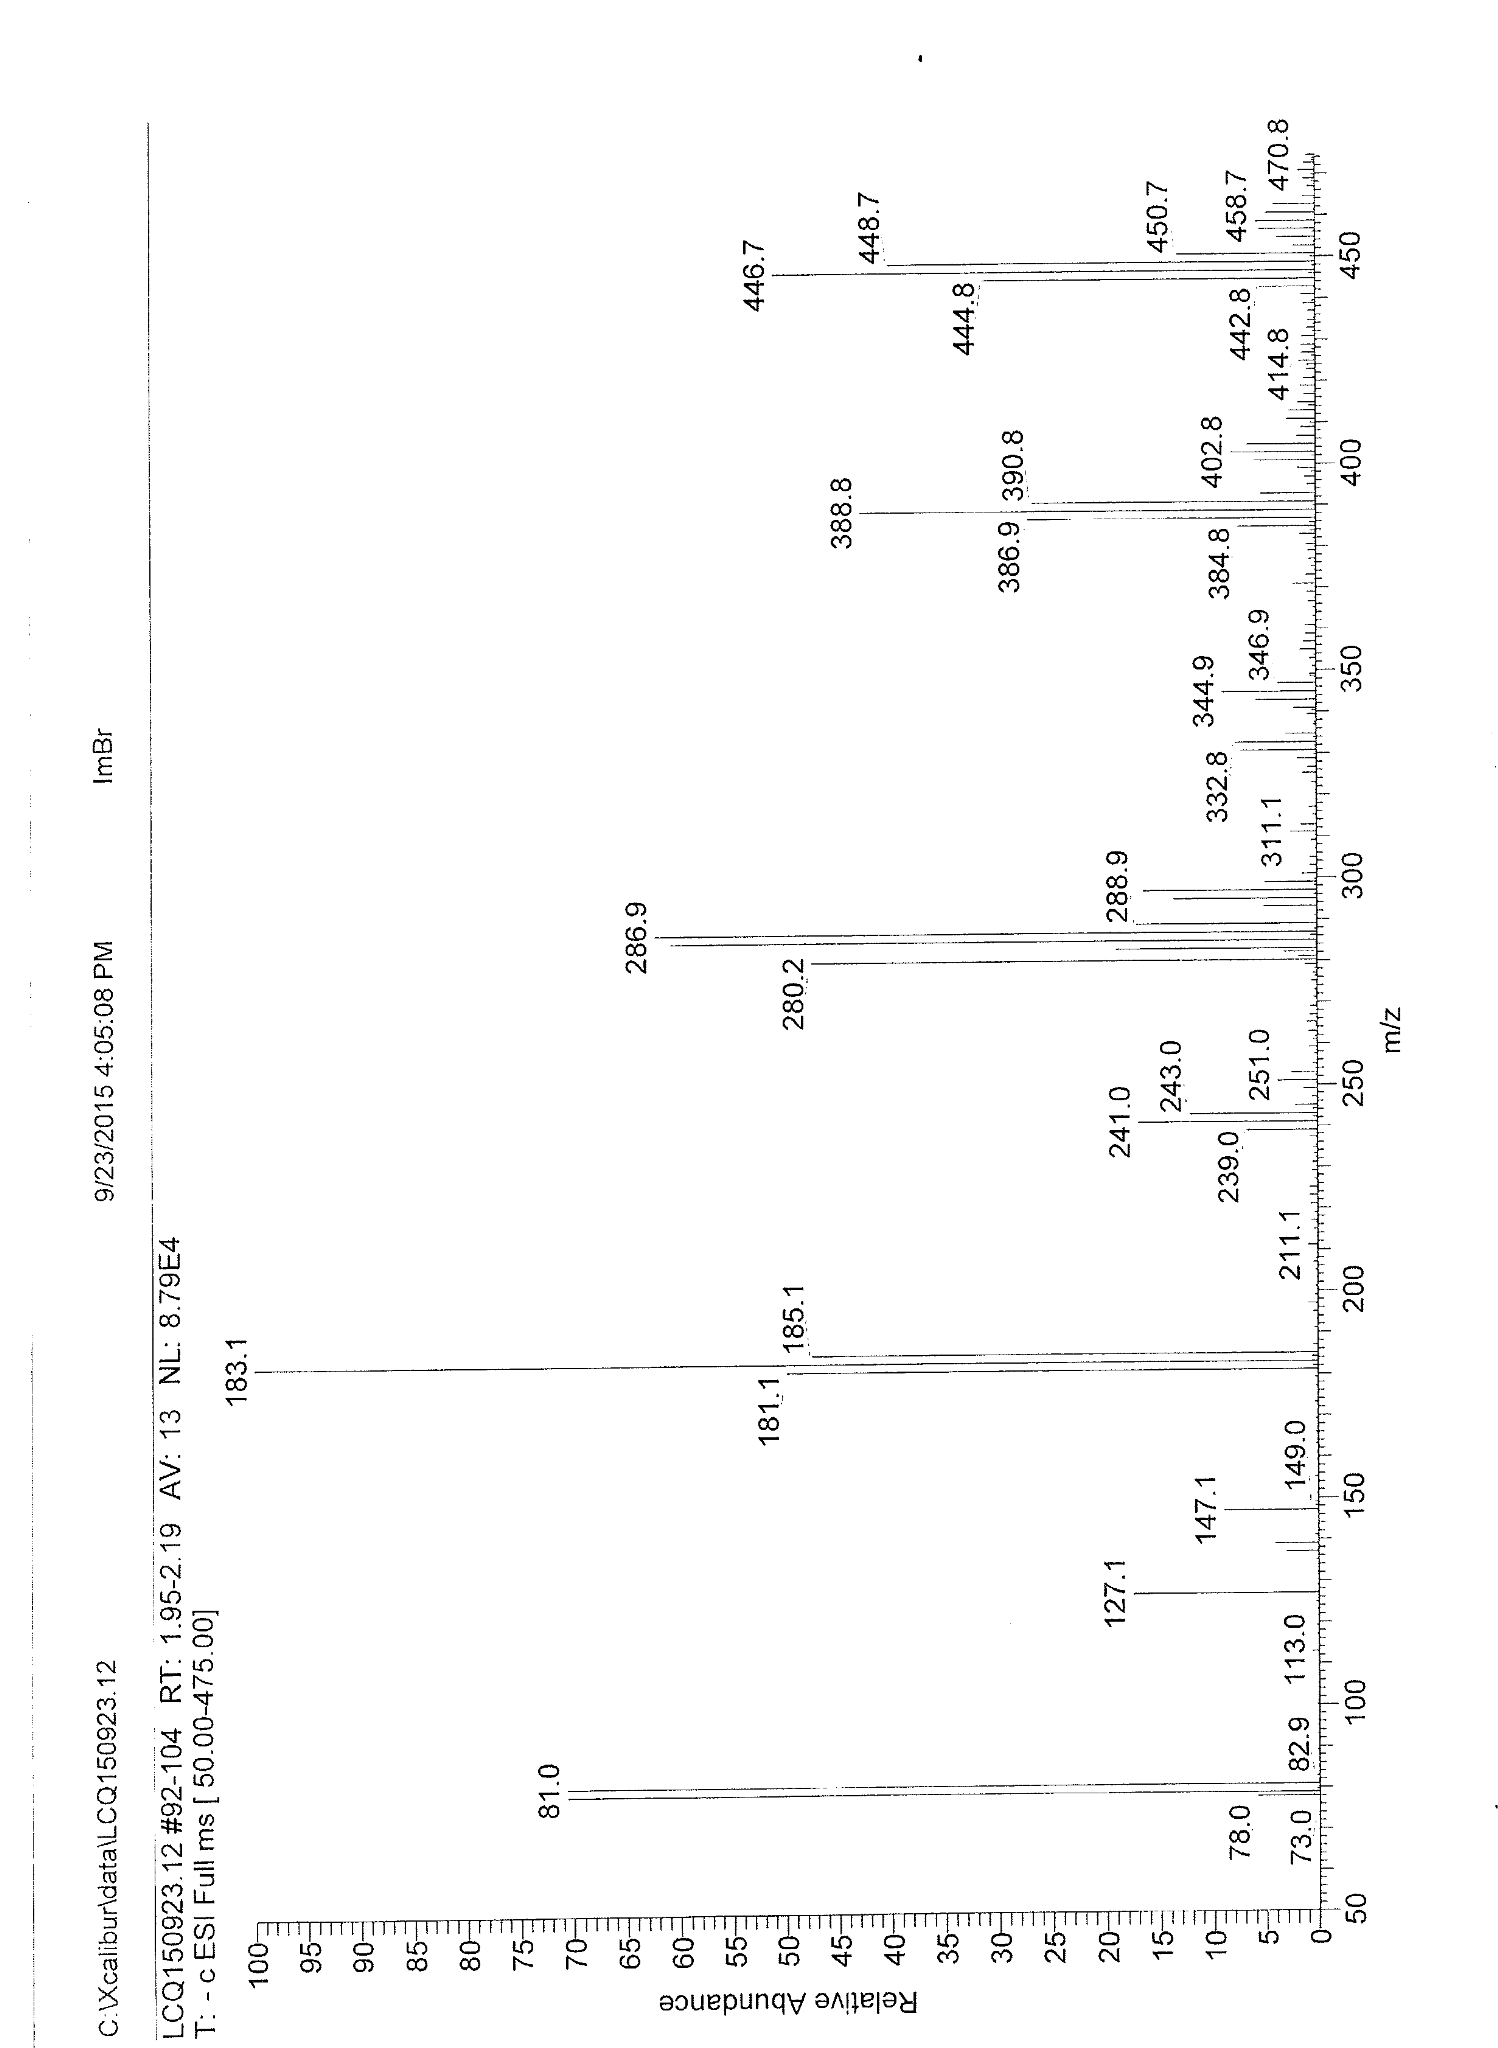
\includegraphics[height=\textheight-2\baselineskip]{mass_PImBr.png}
\caption{High resolution mass spectra of \ce{PIm+Br-}. Bromide peak exist at m/z=81.0.}
\label{fig:massPImBr}
\end{figure}

\begin{figure}
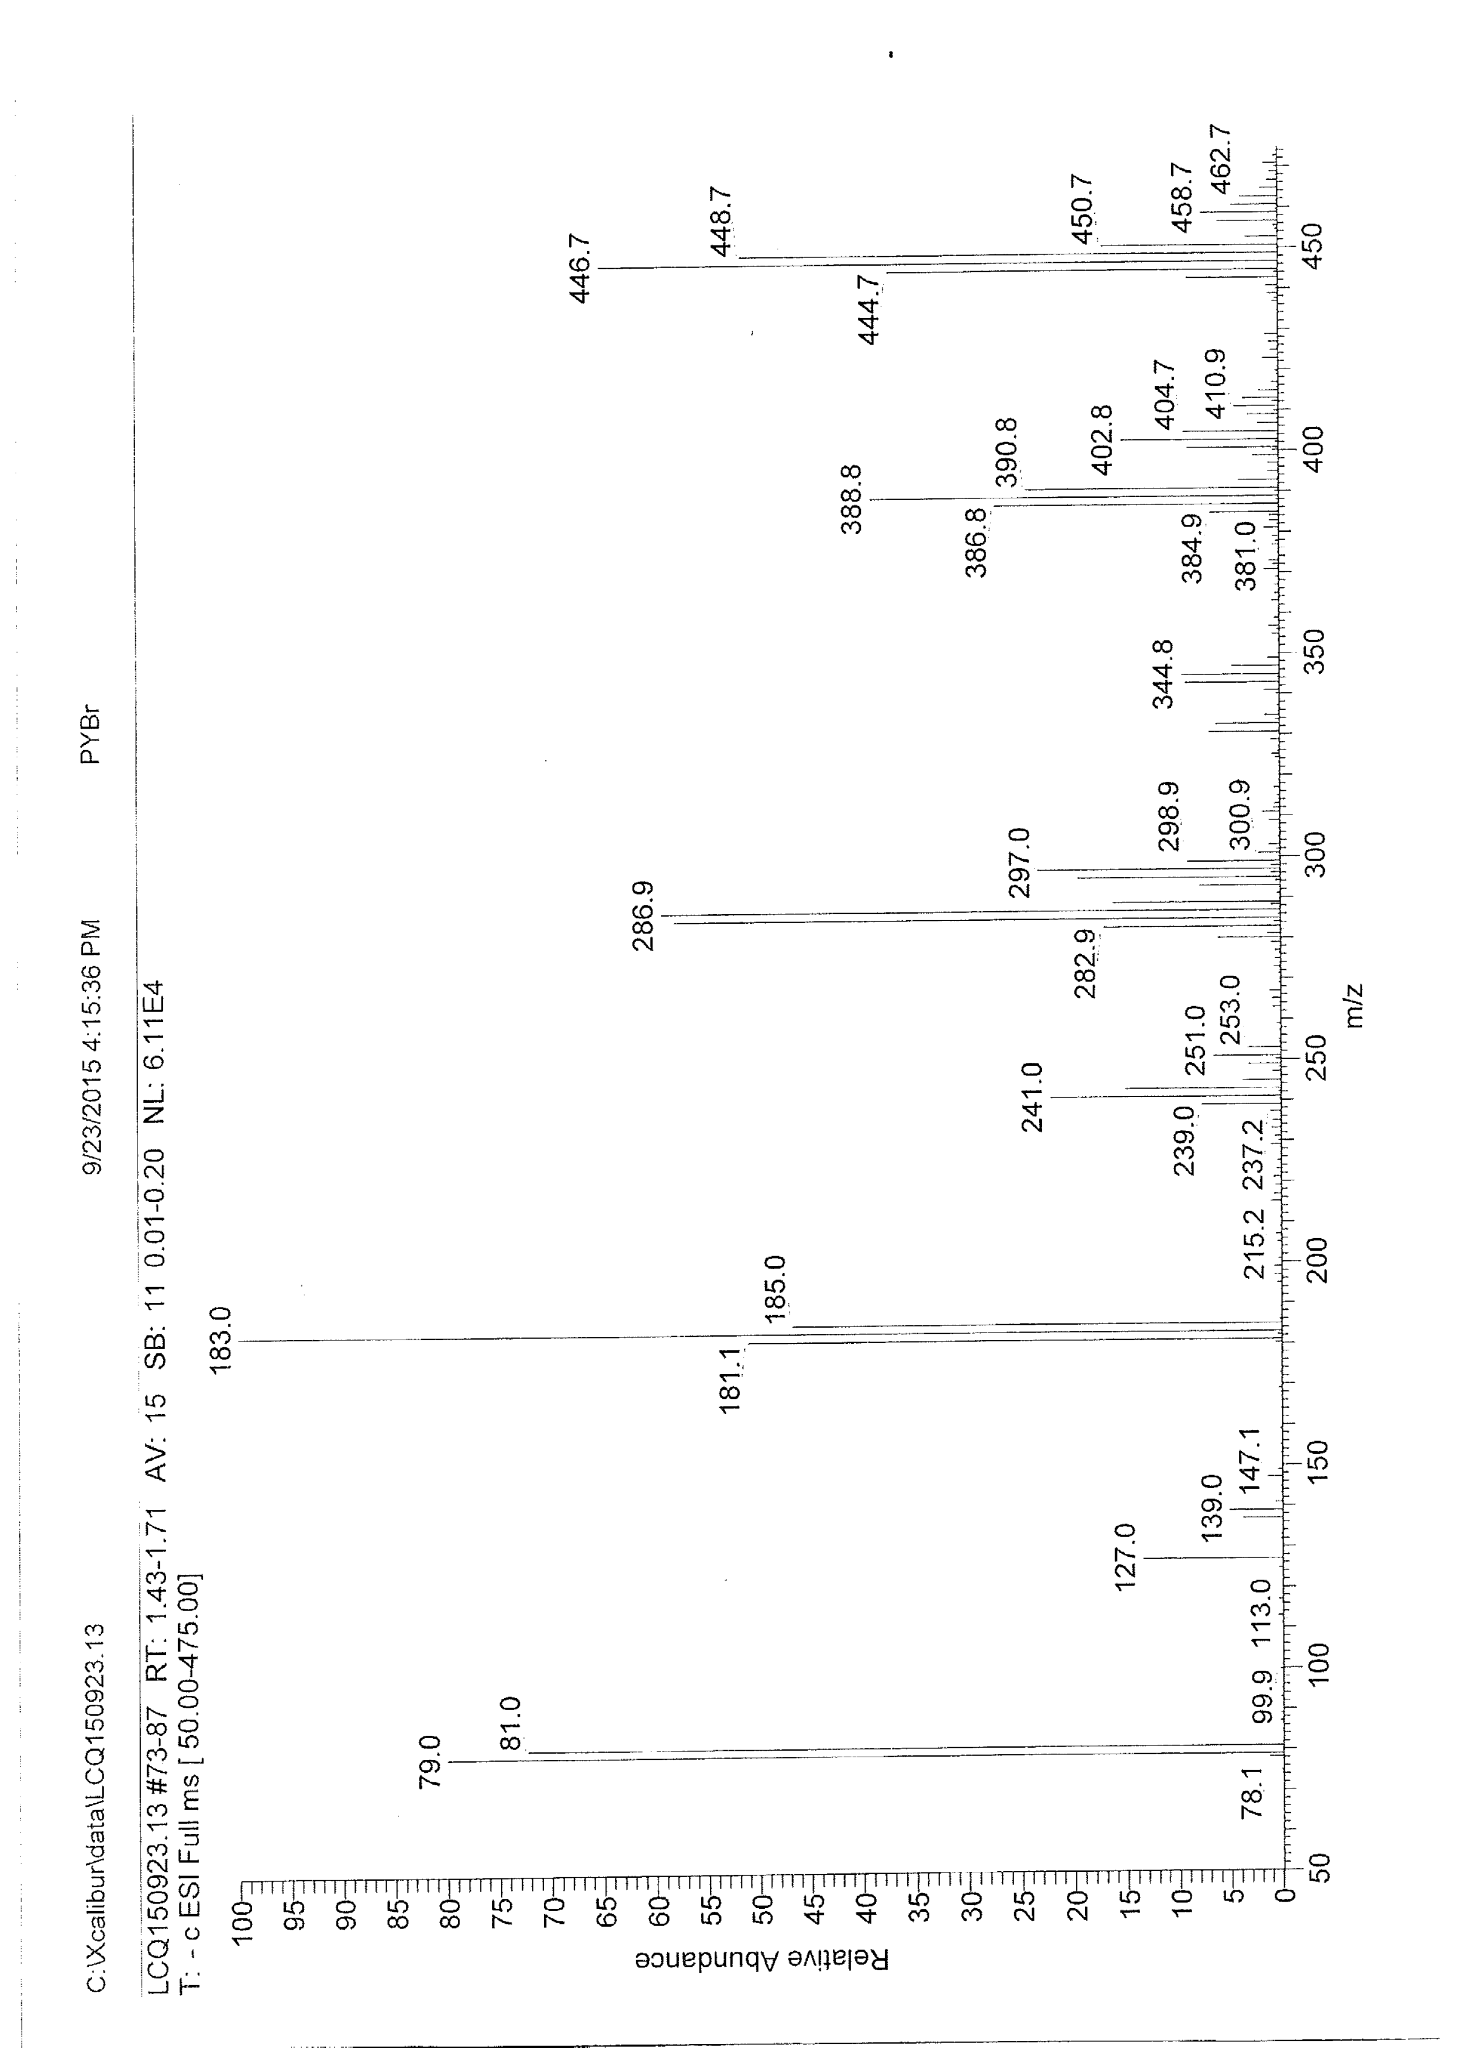
\includegraphics[height=\textheight-2\baselineskip]{mass_PPyBr.png}
\caption{High resolution mass spectra of \ce{PPy+Br-}. Bromide peak exist at m/z=79-81.}
\label{fig:massPPyBr}
\end{figure}

\begin{figure}
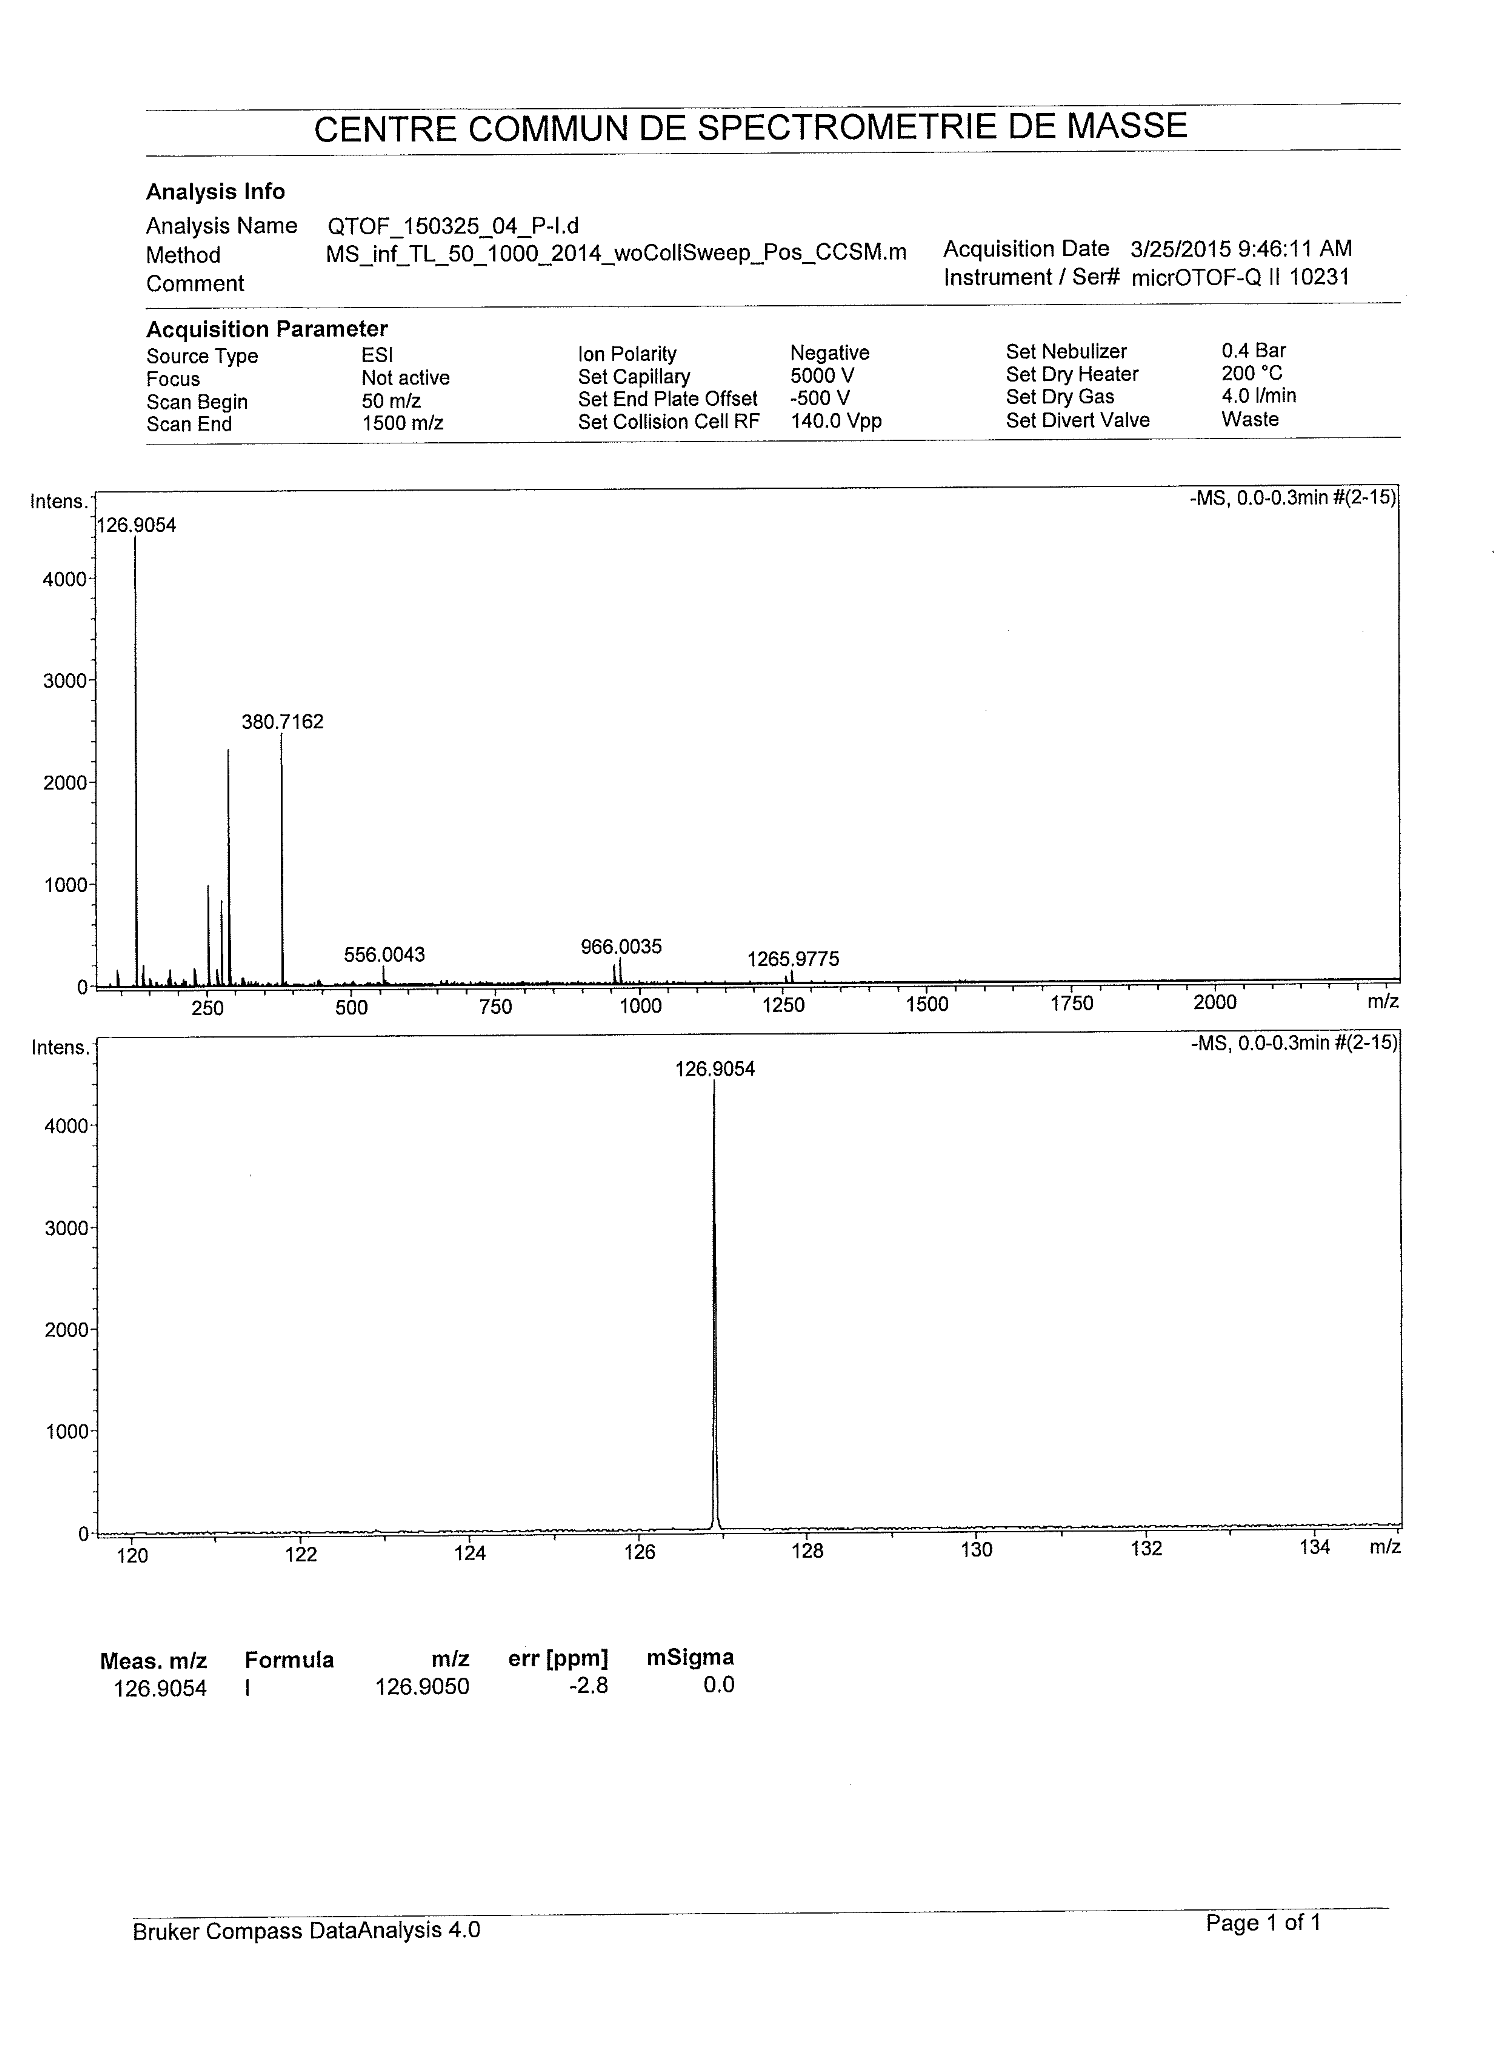
\includegraphics[height=\textheight-2\baselineskip]{mass_PImI.png}
\caption{High resolution mass spectra of \ce{PIm+I-}. Iodide peak exist at m/z=126.9.}
\label{fig:massPImI}
\end{figure}

\begin{figure}
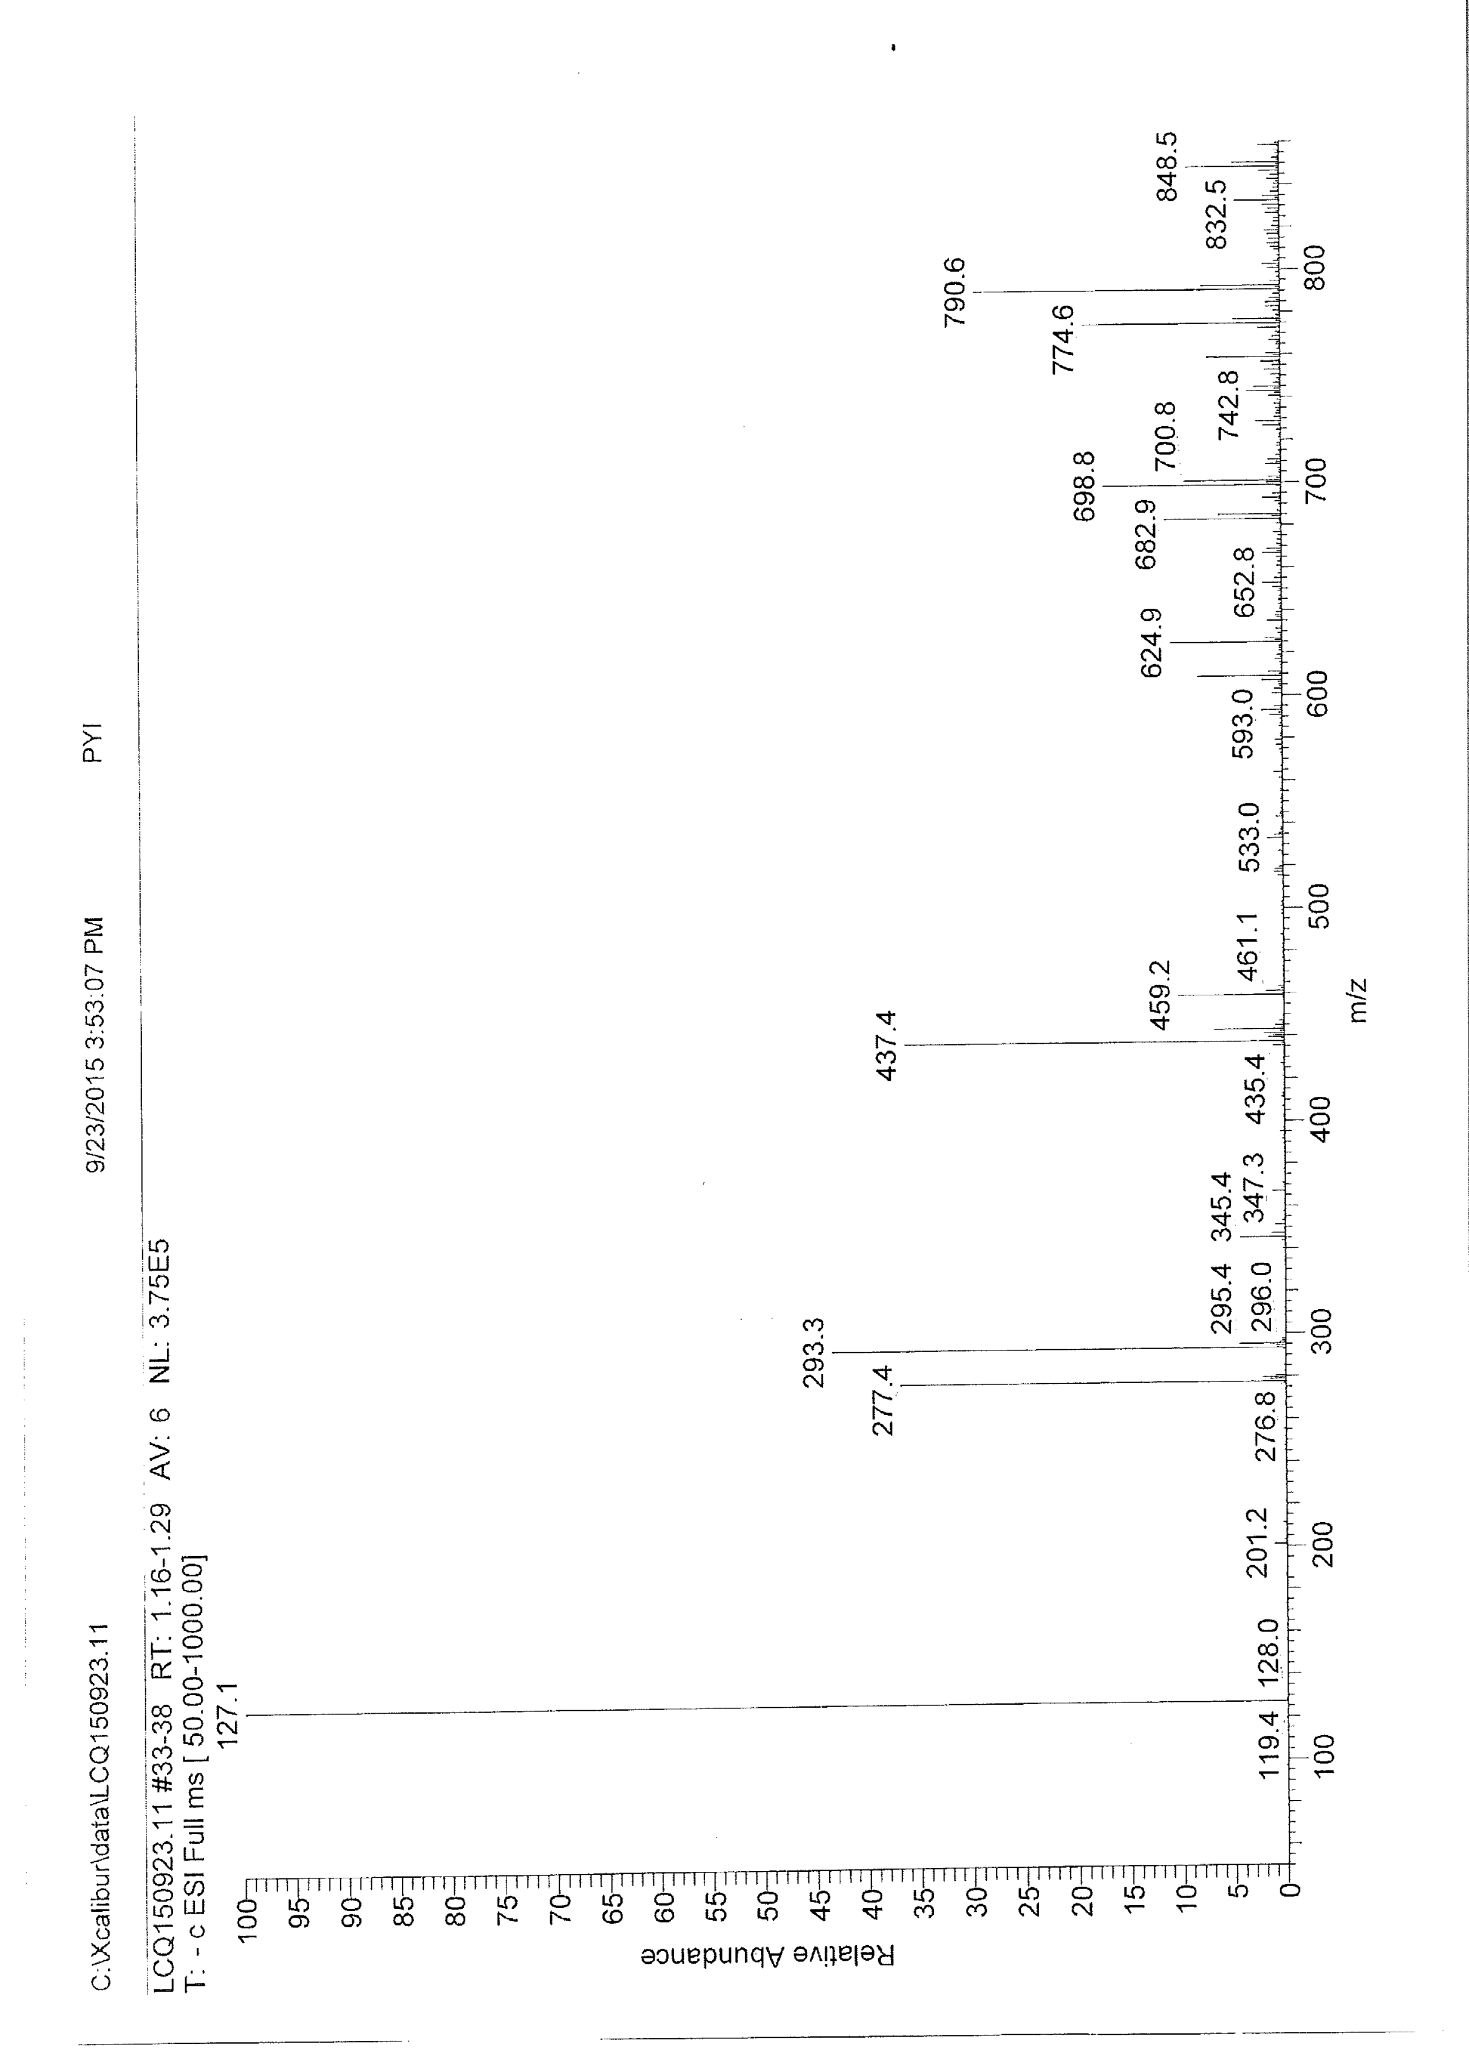
\includegraphics[height=\textheight-2\baselineskip]{mass_PPyI.png}
\caption{High resolution mass spectra of \ce{PPy+I-}. Iodide peak exist at m/z=127.1.}
\label{fig:massPPyI}
\end{figure}

\begin{figure}
\includegraphics{frequency.pdf}
\caption{Storage modulus $G^\prime$ (filled symbols) and loss modulus $G^{\prime\prime}$ (open symbols) measured through oscillatory shear experiments plotted against the frequency $f$ for (a) \ce{PPyr+Cl-} (\textcolor{lightgray}{$\bullet$}), \ce{PPyr+Br-} (\textcolor{gray}{$\blacksquare$}) and \ce{PPyr+I-} ($\blacktriangle$), (b) \ce{PIm+I-} ($\blacktriangledown$) and \ce{PPyr+I-} ($\blacktriangle$) and (c) \ce{PIm+Br-} (\textcolor{gray}{$\blacklozenge$}) and \ce{PPyr+Br-} (\textcolor{gray}{$\blacksquare$}). The fixed strain amplitude is frequency $\gamma=0.1\%$. All samples are at 8\%wt }
\label{fig:frequency}
\end{figure}

\end{document}